% Chapter 2
\chapter{Background Information and Theory} 
\label{Chapter2} 


%----------------------------------------------------------------------------------------
\section{Literature Review} \label{litreview}
% literature review is a paper or article you might sit down to read that gives a general overview of a field. someone not experienced in topic modelling should come a way with a greater understanding of topic models after reading it. And be ready to understand more of your project. 
% explain here what we are going to cover in the literature review.

In this section we begin by reviewing a few of the tasks common in topic modeling. Then we describe a handful of the ways the quality of topic models, LDA in particular, are commonly tested. Finally we discuss the specific tasks of document classification and clustering in the context of topic modeling, as well as the corresponding methods for evaluating model performance at these tasks. 

\subsection{Applications of Topic Modeling}
%------General---------
The most popular application of topic models is simply summarizing large text collections by mining the topics. This is a task LDA is particularly suited for \parencite{griffiths_steyvers04, Mei:2007:ALM:1281192.1281246}. The original LDA paper however \parencite{Blei:2003:LDA:944919.944937} gave promising results on document classification as well. Since then LDA has been used with success not only for document classification, but also for clustering and information retrieval \parencite{Wei:2006:LDM:1148170.1148204, Nagwani2015}. This is due to the strength of the topic vectors LDA models provide, which tend to correlate strongly with human judgement. 

%Though significantly less work has been done assessing the efficacy of LDA extensions such as the DTM and DIM in these areas. 

\subsection{Ensuring Model Quality}
%------Methods of Testing------
\subsubsection{Perplexity Testing}
In order to ensure the strength of these topic vectors researchers employ a handful methods to evaluate the topic models. While the most intuitive method is simply to have humans judge the coherence of each topic, this becomes prohibitively time consuming and expensive for large data sets. One commonly used method of automating this process is by evaluating the topic model on a held out set of testing documents and obtaining the log-likelihood perplexity of the unseen documents \parencite{Blei:2003:LDA:944919.944937, wallach-murray-rsalakhu-mimno-2009}. A higher likelihood on unseen documents, and a lower perplexity score indicates a better model. However this method of evaluating topic model performance has several issues. Firstly, it has been shown that predictive likelihood, or equivalently perplexity, is not always correlated with human judgement, and in some cases is even slightly anti correlated \parencite{Chang:Boyd-Graber:Wang:Gerrish:Blei-2009}. Secondly this method of evaluation only acts as a general measure of the entire model. What about the quality of the individual topics?


% Prior testing of the DTM and DIM specifically, is also based on held out likelihood or perplexity, which as we've mentioned doesn't always correlate with human judgements \parencite{Chang:Boyd-Graber:Wang:Gerrish:Blei-2009}. This leaves considerable room for the exploration and evaluation of both the DTM and DIM on the aforementioned tasks of document classification and clustering.

%DIM involves correlating influences with citation, we replicate and extend by adding page rank

\subsubsection{Coherence Testing}
%------Coherence Testing--------
%why are we not using tfidf?
Fortunately several methods of evaluating the coherence of individual topics from topic models exist. For a topic $t$ we define the \keyword{Umass} coherence as a sum of the pairwise scores of that topic's top words  $W_t =  \{w1, ... w_n\}$. 

\begin{align*}
\text{Umass Coherence } c(t,W_t) &= \sum_{w_i,w_j \in W_t} \text{score}(w_i,w_j) \\
&= \sum_{w_i,w_j \in W_t} log \frac{d(w_i,w_j) + \epsilon}{d(w_i)}
 \numberthis \label{eq:coherence} 
\end{align*}

Where $d(w_i)$ is the number of documents containing the word $w_i$ and $d(w_i,w_j)$ is the number of documents containing both word $w_i$ and $w_j$. The $\epsilon$ in the numerator is simply to smooth the counts and is typically set to a minimal value such as 1 or .01. Intuitively then, a topic is good if its words cooccur often \parencite{Mimno:2011:OSC:2145432.2145462}.

The \keyword{UCI} measure introduced by \parencite{NewmanBB11}, operates in the same manner as Umass but with the pointwise mutual information as a scoring function instead, given in eq \ref{eq:uci}.

\begin{align*}
\text{UCI Coherence } = c(t,W_t) &= \sum_{w_i,w_j \in W_t} \text{score}(w_i,w_j) \\
&= \sum_{w_1,w_2 \in W_t} log \frac{p(w_i,w_j)}{p(w_i)p(w_j)}
 \numberthis \label{eq:uci} 
\end{align*}

Where $p(w_i)$ is the probability of seeing word $w_i$ in a random document and $p(w_i,w_j)$ is the probability of seeing both word $w_i$ and word $w_j$ together in a random document. It should be noted that obtaining these probabilities requires empirically estimating them from an external dataset. 

Two more noteworthy measures of topic coherence, in addition to those outlined above, were developed by Roder, Both and Hinneberg in their study titled "Exploring the Space of Topic Coherence Measures" \parencite{Roder:2015:EST:2684822.2685324}. These measures were the  \keyword{C$\_$v} and \keyword{C$\_$npmi} measures which demonstrated a substantial correlation with human judgement. For brevity we do not replicate their derivations here, but the interested reader will find a detailed description of each in \parencite{Roder:2015:EST:2684822.2685324}

%In a series of experiments on on word sets generated form English and German Wikipedia articles, one study found that a baseline "one-vs-all" approach often outperformed the Umass coherence measure \parencite{DBLP:journals/corr/RosnerHRNB14}.


\subsection{Document Classification}
\label{classificationmetrics}
%------Text Classification---------
Though the topics produced by topic models are useful in their own right for the qualitative analysis of documents, they are also useful quantitatively when trying to classify documents. For instance a large news organization may want to automatically sort its thousands of articles into the categories "politics", "natural disasters" and "sports". To do this they might use a topic model to get a vector of topic proportions for each document to use as features for a classification algorithm. This process is referred to as document vectorization.

% could use tfidf but LDA is sometimes better
While baseline methods for document vectorization exist, such as the Term Frequency Inverse Document Frequency (tf-idf), LDA has been shown to outperform them in certain scenarios. For instance when less training data is available LDA boasted a shorter training time and higher classification accuracy  \parencite{liempirical}. Additionally when tested against other baseline methods for document vectorization such as the unigram model or probabilistic latent semantic analysis (PLSA), LDA again proved consistenlty more accurate at document classification tasks \parencite{Lu:2011:ITP:1969504.1969510}. 

\subsubsection{Accuracy}
When it comes time to evaluate a model's classification performance there are several approaches, the most intuitive of which is accuracy. Accuracy is defined as  

\begin{align*}
acc = \frac{Tp + Tn}{Tp + Tn +Fp + Fn}
 \numberthis \label{eq:acc} 
\end{align*}

Where $Tp$ are our true positives, $Tn$ are our true negatives, $Fp$ are our false positives, and $Fn$ are our false negatives. It should be noted that normal values of accuracy for classification tasks depend highly on the data at hand. Noisy data or a large number of classes can both artificially drive accuracy scores down. 

\subsubsection{Precision}
But what if we want to know, out of the total number of guesses for a particular class, what fraction were correct? For this, researchers typically use the Precision, defined as

\begin{align*}
p = \frac{Tp}{Tp + Fp}
 \numberthis \label{eq:precision} 
\end{align*}

\subsubsection{Recall}
Conversely, if we wish to know out of the total number of cases we could have guessed correctly, what fraction we \emph{did} guess correctly then Recall is typically used. Recall is defined as

\begin{align*}
r = \frac{Tp}{Tp + Fn}
 \numberthis \label{eq:recall} 
\end{align*}

\subsubsection{F1 Score}
The F1 score is a way of combining the above two metrics Precision and Recall into one wholistic measure. Conceptually it is the harmonic mean of the Precision and Recall where we assign even weights to each. The F1 score is defined as


\begin{align*}
F_1 &= \frac{1}{\frac{1}{2}\big( \frac{1}{p} + \frac{1}{r}} \\
&= \frac{2pr}{p+r}
 \numberthis \label{eq:f1} 
\end{align*}

%Again though, prior work indicates no testing of either DTM or DIM in this regard, both of which offer improvements in the latent semantic representation of ordered document collections.

\subsection{Document Clustering}
\label{DocumentClustering}
%------Clustering-------
Another well established task for topic models is document clustering. LDA has been used to successfully cluster a range of documents such as news articles and legal judgements \parencite{Lu:2011:ITP:1969504.1969510, DBLP:journals/corr/XieX13, Kumar2013}. As opposed to classification where we want to assign an explicit label to each document, with clustering we wish to evaluate how well the resulting document topic vectors separate the documents into a meaningful structure.

\subsubsection{Adjusted Rand Score}
One way of accomplishing this is by using the \keyword{Adjusted Rand Score} which measures the similarity of two sets of class labels; namely the true labels $C$ and those predicted by a clustering algorithm $K$. We may calculate the raw (unadjusted) Rand index following equation \ref{eq:RI} \parencite{Hubert1985}. 

\begin{align*}
RI = \frac{a + b}{C_2^{n_{\text{samples}}}}
 \numberthis \label{eq:RI} 
\end{align*}

Where $a$ is the number of pairs of elements in $C$ belonging to the same class, and in $K$ belonging to the same class. Conversely $b$ is the number of pairs of elements in $C$ belonging to different classes, and in $k$ belonging to different classes. Finally, $C_2^{n_{\text{samples}}}$ is the total number of possible pairs in the dataset. In order to ensure that random labelings receive a score of zero we define the adjusted Rand index as 

\begin{align*}
ARI = \frac{RI - E[RI]}{max(RI) - E[RI]}
 \numberthis \label{eq:ARI} 
\end{align*}

\subsubsection{Normalized Mutual Info}
The Normalized Mutual Info is another method of evaluating clustering performance that has been successfully applied in the context of topic modelling \parencite{Xu:2003:DCB:860435.860485, Cai:2008:MHT:1458082.1458202}. It again assumes we have two sets of labels, this time we call them $U$ and $V$, over $N$ objects. We define the entropy of a label set $U$ in equation \ref{eq:entropy}, where $P(i) = |U_i|/N$ is the probability that a random object from $U$ falls into class $U_i$.

\begin{align*}
H(U) = \sum_{i=1}^{|U|} P(i)log(P(i))
 \numberthis \label{eq:entropy} 
\end{align*}

The mutual information (MI) between $U$ and $V$ can be expressed as 

\begin{align*}
MI(U,V) = \sum_{i=1}^{|U|} \sum_{j=1}^{|V|} P(i,j)log(\frac{P(i,j)}{P(i)P(j)})
 \numberthis \label{eq:MI} 
\end{align*}

With these two components we can write the normalized mutual information as proposed in \parencite{Vinh:2009:ITM:1553374.1553511}.

\begin{align*}
NMI(U,V) = \frac{MI(U,V)}{\sqrt{H(U)H(V)}}
 \numberthis \label{eq:NMI} 
\end{align*}

%\subsubsection{Homogeneity, Completeness and V-measure}


%----------------------------------------------------------------------------------------
\section{DTM Model Overview}

% Roadmap + Disclaimer
This section briefly outlines the dynamic topic model (\keyword{DTM}), following closely the original derivation found in \parencite{Blei:2006:DTM:1143844.1143859}. As this is intended as more of a summary, we recommend the reader examine the original paper for a complete exposition of the mechanics of the DTM. 

% Intuition + Conceptual Basis
In our primer on LDA (in section \ref{ldaprimer}) we outlined the conceptual basis for static LDA topic models. Namely, that topics consist of a distribution over a fixed vocabulary and are determined by a set of hyper-parameters $\beta$. Additionally each document is represented as a combination of topics, with proportions controlled by their corresponding set of hyper-parameters $\alpha$. Roughly speaking, the goal of the Dynamic Topic Model (\keyword{DTM}) is to account for the drift in topics over time by chaining together a series of static LDA models. This is accomplished by tying the hyper-parameters $\alpha_{t-1}, \beta_{t-1}$ at time step $t-1$, to the hyper-parameters $\alpha_{t}, \beta_t$ at time step $t$. The result is a model that allows us to track how our topics evolve at each time step. 


%The general approach is to chain together the underlying topic multinomials and topic proportion distributions, then to make use of the Kalman filter to carry out approximate posterior inference over the latent topics.

% how do we actually tie these hyper parameters together?
%With regular latent dirichilet allocation we normally use a Dirichilet distribution to model our uncertainties in word distributions, hence the name. However, this is no longer an option as the Dirichilet distribution does not permit sequential modeling. 

\subsection{Chaining models together}

The question then, is how do we tie our hyper-parameters together? Well, regularly with static LDA we would simply use a Dirichilet distribution to model our uncertainties in word distributions (hence the name). Unfortunately, the Dirichilet distribution does not lend itself to sequential modeling, which eliminates this option. Instead, we make a state-space model that evolves with Gaussian noise to chain together the natural parameters of each topic $\beta_{z,t}$ such that each topic "evolves" from the last.

\begin{align*}
\beta_{z,t} | \beta_{z,t-1} \sim  \mathcal{N}(\beta_{t-1,z},\sigma^2I)  \numberthis \label{eq:topicwordschain} 
\end{align*}

Similarly, with static LDA we would also pull our document specific topic proportions $\theta$ from the Dirichilet distribution. For the same reason as above this is no longer an option. So to express our uncertainty over our topic proportions, we use a logistic normal with mean $\alpha$. Then we chain our topic proportions together using the same trick as we did above with word distributions, (by using Gaussian noise). This yields the graphical model in figure \ref{fig:DTMGM}.

\begin{align*}
\alpha_{t} | \alpha_{t-1} \sim  \mathcal{N}(\alpha_{t-1},\delta^2I)  \numberthis \label{eq:topicpropschain} 
\end{align*}

\begin{figure}[ht]
\centering
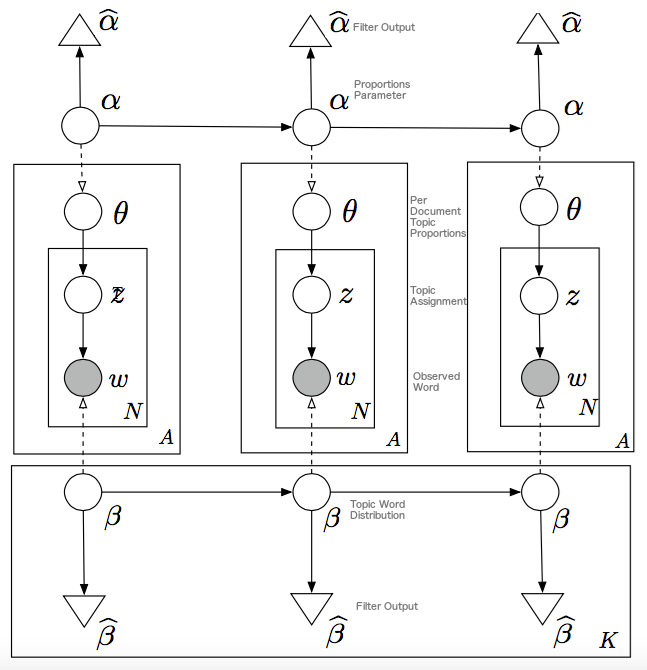
\includegraphics[width=130mm,scale=0.45]{Figures/DTMGM}
\caption[DTMGM]{Graphical model for DTM showing a series of chained static LDA models. The triangles represent the Kalman filter estimates of the hyper-parameters}
\label{fig:DTMGM}
\end{figure}

% could put in the new process from Blei here but maybe that's a bit too much like plagiarism? Would not be cool. 

\subsection{Variational approximate inference}
% motivating variational methods
Because we have used the Gaussian distribution to model the progression of our parameters, inference becomes intractable due to the non-conjugacy of Gaussian and multinomial models. To get around this we take the same variational approach to approximate inference as before in section \ref{ldaprimer} with static LDA. Taking a variational approach has the advantage of allowing us to handle larger document sets compared to Gibbs sampling which becomes computationally difficult at large corpus sizes. 

% variational methods
The general strategy of variational approximate inference is to use a carefully tuned 'approximate' distribution as a substitute for the true posterior. To tune this approximate distribution we minimize the KL divergence between our estimated and true posterior. Finally we may then use this approximated posterior distribution to perform inference.

We begin by creating a collection of variational parameters we will optimize over our latent variables. Our latent variables are the topics $\beta_{t,k}$, topic proportions $\theta_{t,d}$, and topic indicators $Z_{t,d,n}$. While we have variational parameters for each topic (consisting of a sequence of multinomial parameters), and for each document (the latent topic proportions). The resulting posterior, again following the notation of \parencite{Blei:2006:DTM:1143844.1143859} is given by equation \ref{eq:dtmpost}.

\begin{align*}
& \prod_{k=1}^K q(\beta_{k,1}, ... , \beta_{k,T} | \hat{\beta}_{k,1}, ... , \hat{\beta}_{k,T})  \times     \\
& \prod_{t=1}^T \Big( \prod_{d=1}^{D_t} q(\theta_{t,d})| \gamma_{t,d}) \prod_{n=1}^{N_{t,d}}q(z_{t,d,n}|\phi_{t,d,n})   \Big)  \numberthis \label{eq:dtmpost} 
\end{align*}

This is where we tune our approximate posterior, and specifically the variational observations $\{ \hat{\beta}_{k,1}, ... , \hat{\beta}_{k,T}  \}$ according to the KL divergence between the estimated and the true posterior. Note that here, each topic proportions vector $\gamma_{t,d}$ receives a corresponding free Dirichilet parameter, while each topic indicator $z_{t,d,n}$ receives a corresponding free multinomial parameter $\phi_{t,d,n}$. To optimize the document topic proportion vectors we subsequently employ gradient ascent, however this is not necessary for the document level parameter updates as they simply have a closed form.

%topic tracking
Finally, we may track our variational parameters $\hat{\beta}$ and $\hat{\alpha}$  between time slices using either the Kalman filter or wavelet regression. For brevity we will not replicate the mechanics of these methods here and encourage the interested reader to refer to the derivations provided in detail in  \parencite{Blei:2006:DTM:1143844.1143859}.


%\subsection{Issues}
%The DTM is not without its fallbacks. 
%addresses several latent structures in the document collection such as topic evolution and prevalence, however does not address the birth and death of topics, like models such as \cite{DBLP:journals/corr/abs-1203-3463}.

%--------------------------------------------------------------------------------------
%\section{DIM Model Overview} 

%language based approach to modeling the influence of documents.
%useful when traditional bibliometrics such as citations are not available. produces an internal measure of document influence that has been shown to correlate with citations. Closely related to the DTM but with XXX.

% important for decisions about publishing and funding
% also relevant to know for scientists who should read important work in their field for good research practice

%probability of a word given the natural parameters of the word distribution beta at time t

%then we have as in the DTM a logistic normal markov chain
%(its drift is a stationary autoregressive process)

%central idea: some articles influence the topic more than others.

%initialize normally distributed scalar influence scores $l_d$ to describe the influence article $d$ has on the topic. Higher influences mean a document had a larger affect on the drift of the topic.


%give equation of time series model


%word from documents of high influence will have a higher probability in the following time step while words from an article with zero influence will not affect the next time step. As with the dtm, once trained on our corpus the posterior of topic and influence scores gives gives a trajectory of term fre- quencies and a retrospective estimate of the influence of each article. An article whose words can help explain the way the word frequencies change will have a high posterior influence score

%[image of the graphical model]























